\begin{refsegment}
\chapter{Investigations sur la logique paracohérente}

Comme évoqué précédemment, les données et prédictions en biologie peuvent être incomplètes et contradictoires. Ces trois années de recherche ont été consacrées à la conception d’une méthode et d'un logiciel qui a pour objectif d'aider les biologistes à évaluer les prédictions bio-informatiques pour l'annotation fonctionnelle des génomes au travers de processus biologiques. Un tel système expert doit donc être capable de gérer des annotations inconsistantes d'où le choix d'orienter mes travaux dans le cadre de la logique paracohérente.

\section{Contexte du projet}

Mon projet de recherche a débuté par l'identification des besoins et des outils à ma disposition. Les orientations technologiques de la plateforme \texttt{MicroScope} (i.e. plateforme d’annotation de génomes microbiens, développée dans le laboratoire où j’ai réalisé ces travaux) portaient sur trois axes.

Le premier correspondait à la modernisation du système de gestion et de déclaration des chaînages applicatifs ("wokflows"). Pour cela, la plateforme \texttt{MicroScope} s'oriente vers la mise en place d'un moteur à base de règles développé en interne au \texttt{GenoScope} (\texttt{\gls{BIRDS}}) . Le système utilise l'application \texttt{DROOLS}\cite{mcwhirter2001drools,browne2009jboss} pour raisonner et ordonner les processus à partir de règles métiers décrivant les ressources à utiliser et l’enchainement des programmes dans le processus d'annotation de génomes.

Le second axe consistait à la mise en place d'un système d'intégration des données métaboliques de la plateforme, dénommé \texttt{Galileo} \cite{galileo2014}. Cet outil a la faculté de réconcilier les informations provenant de multiple ressources externes et internes. Les informations contenues dans ces différentes ressources sont réunies dans une interface unique. Les informations sont extraites des ressources \texttt{ChEBI} \cite{hastings2013chebi}, \texttt{RHEA} \cite{alcantara2012rhea}, \texttt{KEGG} et \texttt{MetaCyc}. Ainsi, \texttt{Galileo} permet d'avoir accès à un large éventail d'information sur les connaissances métaboliques. 

Le troisième axe s'articulait autour d'un système à base de règles pour l'annotation des génomes. Il a pour objectif de guider le biologiste sur les annotations suspectées manquantes dans un organisme donné. Il est composé de deux modules. Le premier a pour objectif de récupérer les règles d'\texttt{UniRule} et de les rendre utilisables en dehors de "l'\gls{EBI}". Les règles d'annotations fonctionnelles établies à partir des domaines protéiques seraient ainsi partagées à la communauté scientifique. Le deuxième module doit évaluer les fonctions prédites au regard des processus métaboliques et mettre en évidence des annotations confirmées, manquantes ou contradictoires. La cohérence des annotations d'un génome peut ainsi être évaluée vis-à-vis des attentes portées sur des processus que l'organisme est capable de réaliser. Le moteur de règles \texttt{DROOLS} a été choisi pour la mise en œuvre du raisonnement. Ce moteur est moderne et il est capable de communiquer avec des applications  \texttt{Java} ce  qui est un avantage car \texttt{Galileo} et \texttt{BIRDS} sont également écrits dans ce même langage.

C'est sur ce dernier axe que j'ai effectué mes recherches tout en échangeant avec les deux premiers afin de récupérer les prédictions bio-informatiques et les données métaboliques unifiées. Le contexte de mon projet de recherche a été présenté lors de la 10$^{eme}$ conférence internationale sur l'intégration de données en sciences de la vie (DILS 2014 \url{http://dils2014.inesc-id.pt/}).

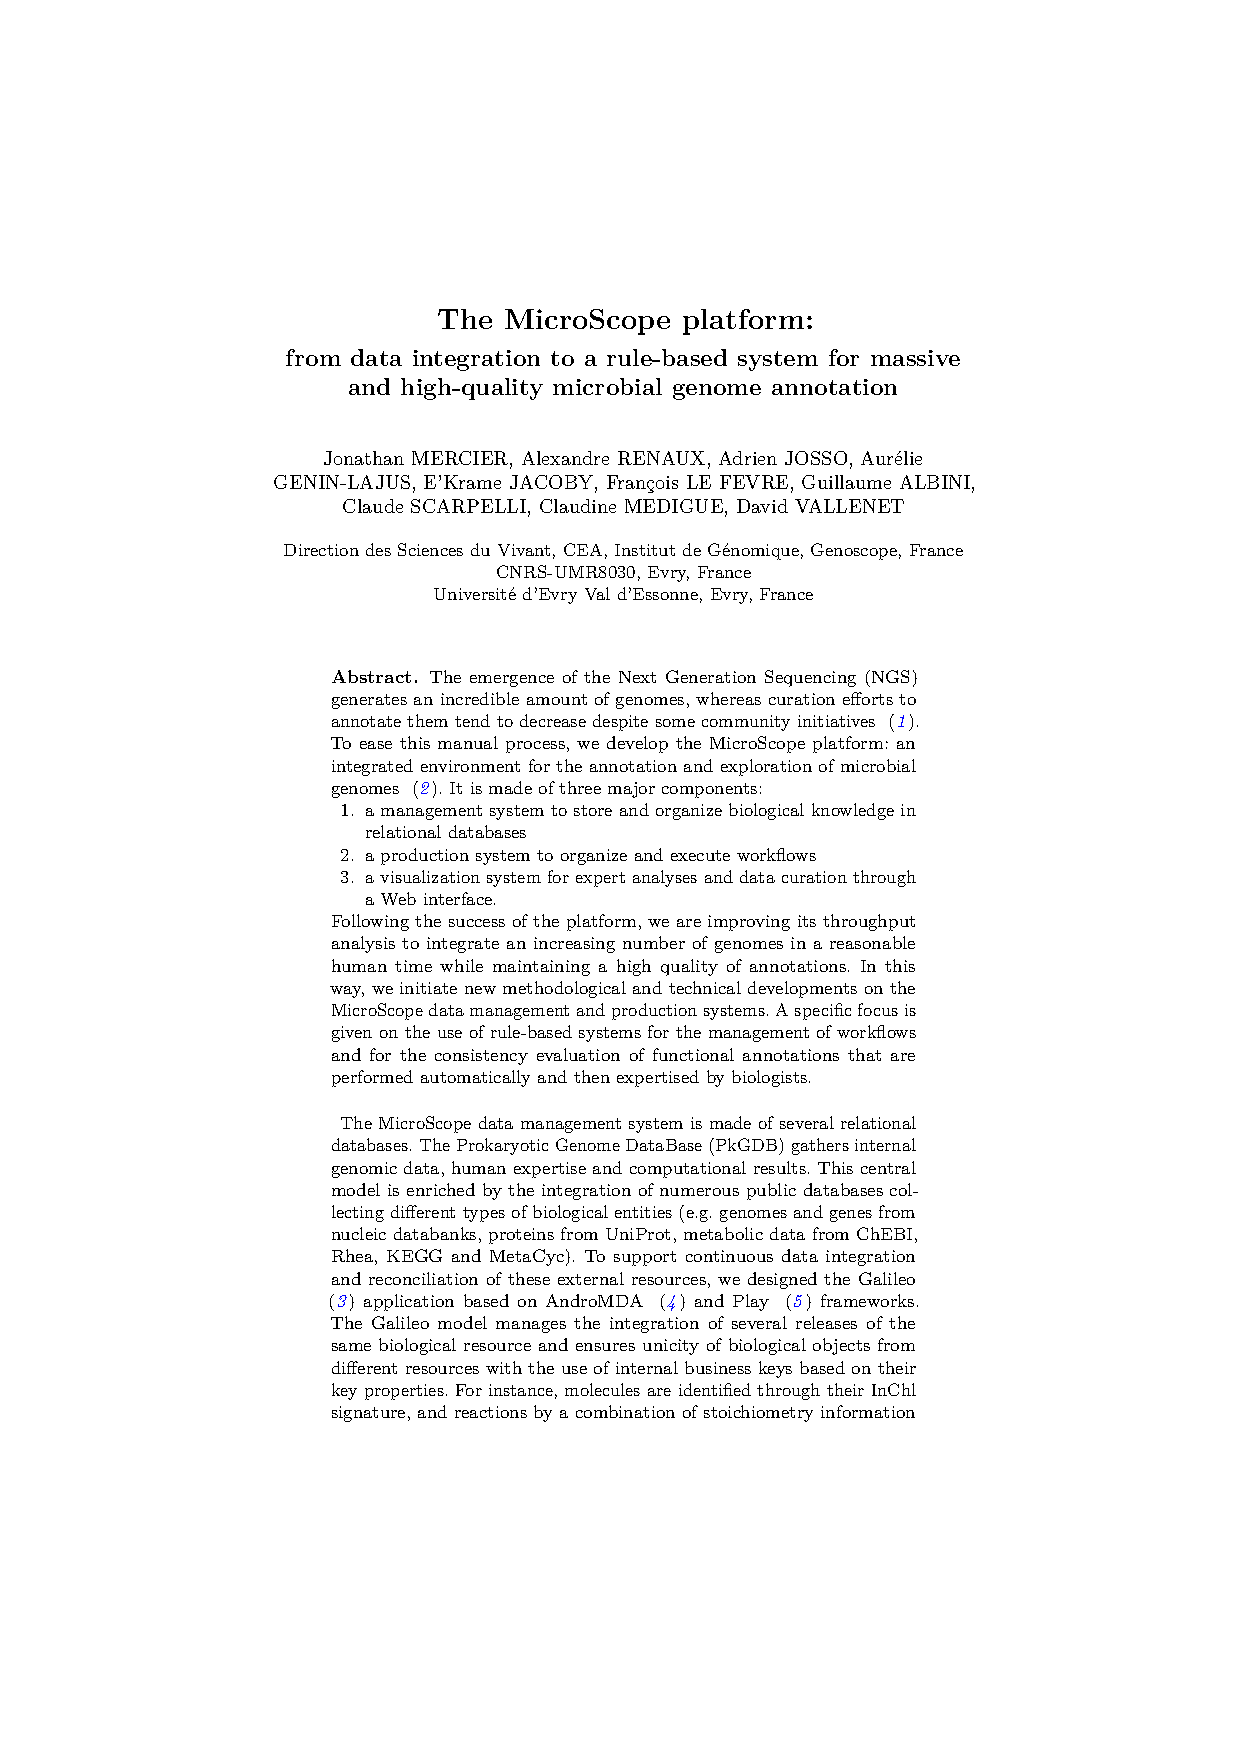
\includepdf[pages=-]{img/DILS_2014.pdf}

\section{HERBS}

L'équipe \texttt{HELIX}, dirigée par \textit{Alain VIARI}, avait commencé un projet en ce sens nommé \texttt{\gls{HERBS}} en collaboration avec le \texttt{\gls{SIB}} dans le cadre du projet \gls{HAMAP} \cite{pedruzzi2015hamap}. L'objectif de \texttt{\gls{HERBS}} est d'alerter les biologistes sur les fonctions et les voies métaboliques manquantes, non attendues ou encore ambiguës. Pour cela, l'outil s'appuie sur le moteur d'inférence \texttt{\gls{JESS}}, sur une base de connaissances (contenant les règles et les faits, \cref{fig:systeme_expert}) et sur une interface graphique pour l'exploration des connaissances. 

Les connaissances dans \texttt{HERBS} sont structurées en trois composants :\nolisttopbreak
\begin{itemize}
    \item La base de connaissance contient des faits primaires sur l’organisme étudié (sa taxonomie  et des propriétés phénotypiques, exemple : l’organisme est photosynthétique) et des faits généraux décrivant des processus biologiques et leurs composants sous la forme d’un  graphe orienté acyclique avec des nœuds \texttt{ET} et \texttt{OU}.
    \item La base d’observations contient des prédictions d’unités fonctionnelles (i.e. composants de processus) dans l’organisme étudié.
    \item Des règles logiques permettant de prendre des décisions (e.g. SI X est requis par une bactérie et X n’est pas observé ALORS X est manquant dans l’annotation de la bactérie).
\end{itemize}

Le raisonnement dans \texttt{HERBS} se fait en propageant les observations au travers du graphe de connaissances par l’application des règles logiques. Chaque nœud est associé à trois attributs pouvant prendre les valeurs "oui" ou "non" au cours du raisonnement :\nolisttopbreak
\begin{itemize}
    \item "Présent", le composant est prédit ou non dans l’organisme
    \item "Requis", le composant est observé dans l’organisme (e.g. un phénotype de croissance)
    \item "Interdit", le composant n’est pas attendu dans l’organisme.
\end{itemize}

À la fin du raisonnement, des conclusions sur les processus et leurs composants sont données suivant cette table de correspondance :\nolisttopbreak
\begin{table}[H]
    \centering
    \label{tab:herbs_conclusion}
    \begin{tabular}{|l|l|l|>{\columncolor{LightCyan}}l|}
        \toprule
        \rowcolor{LightCyan}
        \textbf{Présent} & \textbf{Requis} & \textbf{Interdit} & \textbf{Conclusion} \\ 
        \midrule
        oui & oui & oui & ambigu \\ 
        \hline 
        oui & oui & non & normal \\ 
        \hline 
        oui & non & oui & inattendu \\ 
        \hline 
        oui & non & non & orphelin \\ 
        \hline 
        non & oui & oui & ambigu \\ 
        \hline 
        non & oui & oui & manquant \\ 
        \hline 
        non & non & oui & normal \\ 
        \hline 
        non & non & non & normal \\ 
        \bottomrule
    \end{tabular} 
\end{table}

\textit{Alain VIARI} m'a permis d'utiliser l'outil \texttt{PathRules} qui est une implémentation de \texttt{\gls{HERBS}} avec le moteur \texttt{\gls{CLIPS}} \cite{riley1991clips}. Pour tester ce logiciel, j'ai fourni à la base de faits les voies de biosynthèse de la lysine avec les variants \texttt{AAA} et \texttt{DAP} décrits par \texttt{UniPathway} et les prédictions d’activités enzymatiques provenant de l’analyse de 79 génomes. Pour ce faire, les données sont rangées dans trois dossiers présents à la racine du projet: (i) \texttt{data/processes} pour la description des voies métaboliques, (ii) \texttt{data/observers/uniprot} pour le catalogue des prédictions par espèce, (iii) \texttt{data/species} pour la description taxonomique des espèces. Les fichiers doivent porter l'extension \texttt{.data} et le nom du fichier est utilisé comme identifiant pour faire le lien entre les processus, les prédictions et les informations taxonomiques de l'espèce. Par exemple, j'ai utilisé l'identifiant \texttt{ACIAD} pour mettre en relation les informations d'\textit{Acinetobacter baylyi} ADP1.

\console{find data/ -name 'ACIAD.data'}{ data/observers/uniprot/ACIAD.data\par data/species/ACIAD.data }


La description des données dans ces fichiers suit la nomenclature \texttt{\gls{CLIPS}}, c'est-à-dire que les faits sont déclarés entre parenthèses. C'est la raison pour laquelle les observations sont formatées comme suit: 

( \texttt{source} (id \texttt{xxx}) (alias \texttt{yyy} sp:\texttt{zzz})  )

Extrait d'un fichier cataloguant les faits relatifs à un organisme:\nolisttopbreak

\console{head data/observers/uniprot/data/ACIAD.data}{
    (uniprot (id ASPARTATE-SEMIALDEHYDE-DEHYDROGENASE-RXN) (alias ACIAD0479 sp:ACIAD00423))\par
    (uniprot (id SUCCDIAMINOPIMDESUCC-RXN) (alias ACIAD0791 sp:ACIAD0070)\par
    (uniprot (id ASPARTATEKIN-RXN) (alias ACIAD1252 sp:ACIAD01133))\par
    (uniprot (id SUCCINYLDIAMINOPIMTRANS-RXN) (alias ACIAD2080 sp:ACIAD01886))\par
    (uniprot (id TETHYDPICSUCC-RXN) (alias ACIAD2599 sp:ACIAD02357))\par
    (uniprot (id DIAMINOPIMEPIM-RXN) (alias ACIAD2659 sp:ACIAD02412))\par
    (uniprot (id DIAMINOPIMDECARB-RXN) (alias ACIAD2660 sp:ACIAD02413))\par
    (uniprot (id DIHYDRODIPICSYN-RXN) (alias ACIAD3585 sp:ACIAD03222))\par
    (uniprot (id DIHYDROPICRED-RXN) (alias ACIAD3619 sp:ACIAD03252))\par
}


L'information taxonomique est également un fait. Il débute par le mot-clé "species" suivi de chaînes de caractères de plus en plus précises sur la taxonomie de l'organisme.

\console{cat data/species/ACIAD.data}{ (species lineage Bacteria Proteobacteria Gammaproteobacteria Pseudomonadales Moraxellaceae Acinetobacter Acinetobacter\_baylyi\_ADP1) }

Pour représenter la structure hiérarchique des voies métaboliques, les faits sont organisés pour exprimer la notion de composition et d'équivalence. La notion de composition est utilisée pour relier les ensembles de réactions (\gls{ULS} \texttt{d’UniPathway}) à leurs réactions. Quant à l'équivalence, elle permet de définir les chemins alternatifs (variants) pour réaliser une voie métabolique. La syntaxe \texttt{\gls{CLIPS}} utilise $x -> \ldots$ pour signifier "x tel que \ldots". La partie à droite de la flèche décrit les relations en notation polonaise\footnote{Également connue sous le nom "notation pré-fixée". Par exemple, le calcul "$5 \times (2 + 3)$", s'écrit "$\times 5 (+ 2 \qquad 3)$". }. Ci-après le fichier de description de la voie métabolique de la biosynthèse de la lysine par le variant \texttt{AAA} (Acide alpha-Amino Adipique) selon \texttt{UniPathway}.

\console{cat data/processes/lysine\_AAA\_biosynthesis.data}{
    ;;;; --------------------------------------------------------\par
    ;;; HERBS (Hamap Expert Rules Based System)\par
    ;;;\par
    ;;; @file: lysine\_AAA\_biosynthesis.data\par
    ;;; --------------------------------------------------------\par
    ;;;\par
    (process declare lysine\_AAA\_biosynthesis present in ALL)\par
    (process define lysine\_AAA\_biosynthesis -> and UPA00033)\par
    (process define UPA00033 -> or UPA00033-alt-0 UPA00033-alt-1)\par
    (process define UPA00033-alt-0 -> and ULS00012 ULS00013)\par
    (process define UPA00033-alt-1 -> and ULS00012 ULS00014)\par
    (process define ULS00012 -> and ULS00012-alt-0)\par
    (process define ULS00012-alt-0 -> and UER00028 UER00029 UER00030 UER00031 UER01027)\par
    (process define ULS00013 -> or ULS00013-alt-0 ULS00013-alt-1)\par
    (process define ULS00013-alt-0 -> and UER00032 UER00034)\par
    (process define ULS00013-alt-1 -> and UER00033 UER00034)\par
    (process define ULS00012 -> and ULS00012-alt-0)\par
    (process define ULS00012-alt-0 -> and UER00028 UER00029 UER00030 UER00031 UER01027)\par
    (process define ULS00014 -> or ULS00014-alt-0 ULS00014-alt-1)\par
    (process define ULS00014-alt-0 -> and UER00035 UER00037 UER00038 UER00039)\par
    (process define ULS00014-alt-1 -> and UER00036 UER00037 UER00038 UER00039)\par
}


Chaque processus est un fait, désigné par le mot-clé "process". Les voies métaboliques sont préfixées du mot-clé "declare" et "define" pour ses composants. Les faits constituant la voie métabolique sont hiérarchiquement organisés. Lorsqu'un fait est composé de plusieurs concepts, on utilise le symbole "and" et le symbole "or" lorsqu'un fait possède des équivalences. Les lignes débutant par un point virgule ne sont pas interprétées par \texttt{\gls{CLIPS}}. Elles permettent de commenter les règles et les faits.

À la fin du raisonnement, une évaluation de la complétion de l'annotation fonctionnelle des génomes est proposée sous la forme d’un tableau(\cref{fig:herbs_rapport}).

\begin{shadedfigure}[H]
    \centering
    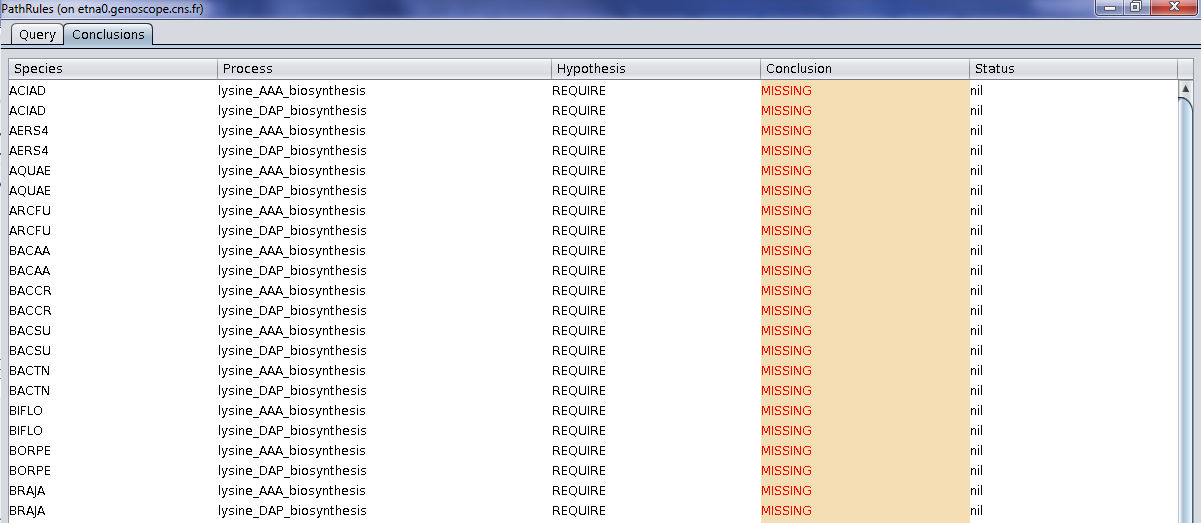
\includegraphics[width=\textwidth]{img/herbs_conclusion_report.png}
    \caption{Rapport sur la présence de la voie de biosynthèse de la lysine.}
    \label{fig:herbs_rapport}
\end{shadedfigure}

L'utilisateur a la possibilité d'explorer les résultats de \texttt{\gls{HERBS}} sur les voies métaboliques et leurs composants à travers un graphe orienté acyclique (\cref{fig:herbs_dag}).

\begin{landscape}
    \begin{shadedfigure}[H]
        \centering
        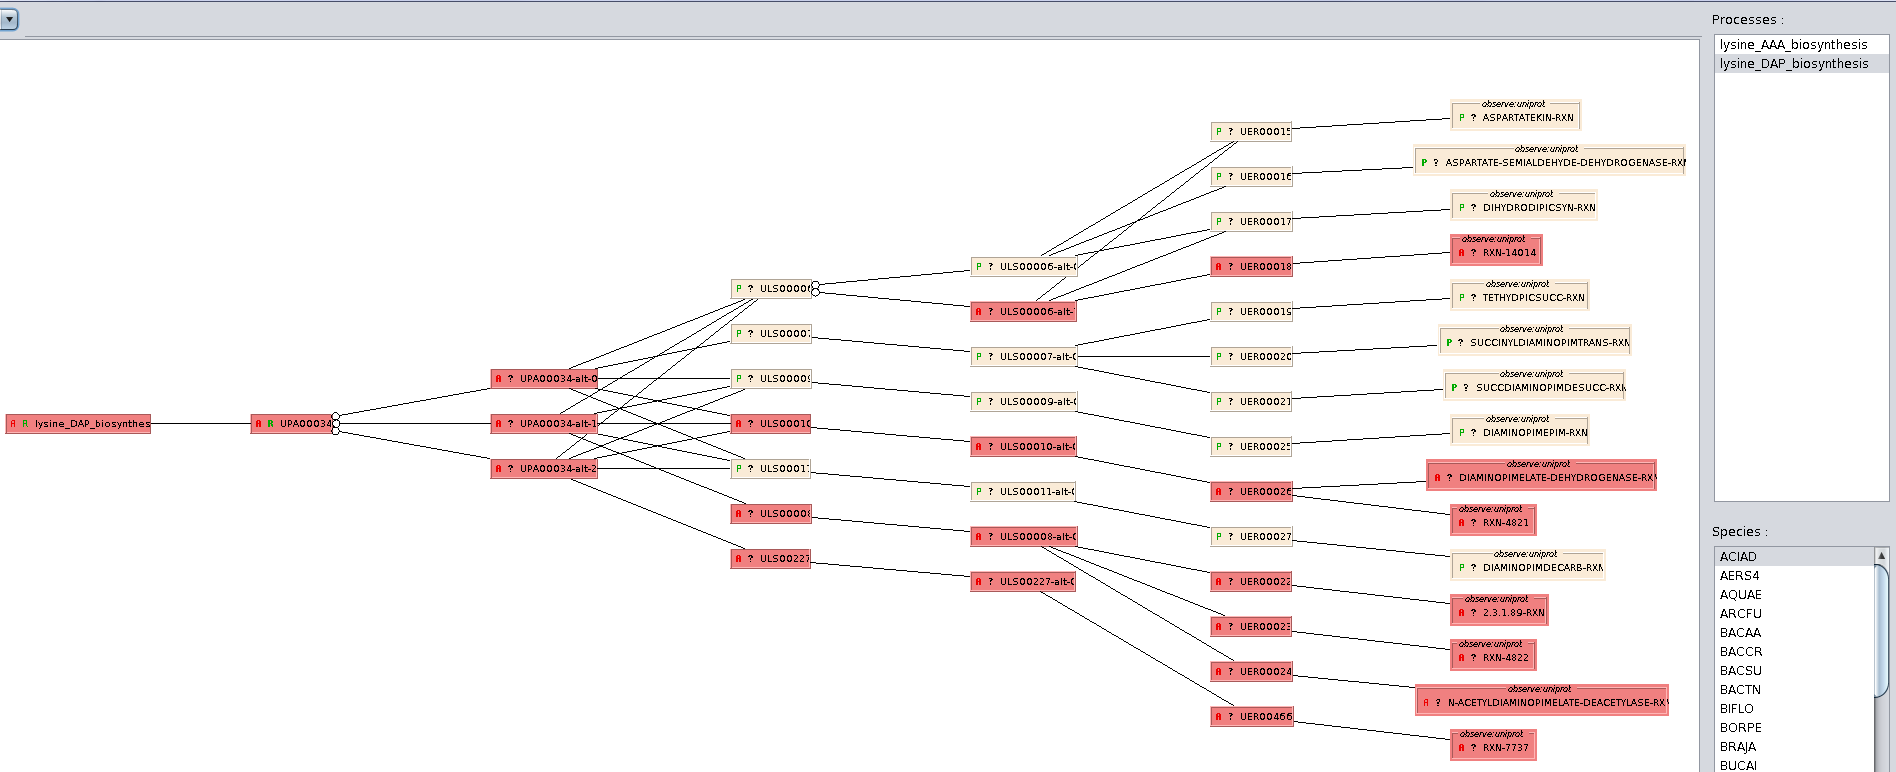
\includegraphics[width=\textwidth]{img/herbs_aciad_lysine_dap.png}
        \caption{Rapport sur la présence de la voie de biosynthèse de la lysine pour un organisme. La couleur jaune indique que la prédiction portée sur le concept est en accord avec les connaissances sur l'organisme. Dans le cas contraire, le concept est sur fond rouge. }
        \label{fig:herbs_dag}
    \end{shadedfigure}
\end{landscape}


Une des difficultés dans l’utilisation de \texttt{\gls{HERBS}} est tout d’abord de traduire toutes les connaissances sur les voies métaboliques et les prédictions en CLIPS. De plus, le système ne prend pas en charge la notion d’inconnu et la contradiction sur les prédictions. En effet, en biologie, l’absence de résultat suite à une expérience ou à une prédiction est souvent difficile à interpréter comme un résultat vrai négatif ou faux négatif. Ce point de vue peut paraître quelque peu philosophique. Il fait référence aux concepts de "monde ouvert" et "monde fermé". Une hypothèse en monde fermé va considérer toutes les questions sans réponse comme fausses. En monde ouvert, les hypothèses prennent la valeur vrai ou faux lorsqu'elles sont explicitement décrites comme telles. Pour les autres cas, une hypothèse est considérée incertaine tant qu'un fait ne la désigne pas comme vraie ou fausse. Dans l’exemple précédent de \texttt{\gls{HERBS}}, la plupart des voies métaboliques sont déclarées "Missing" sans pour autant suggérer quel variant est le plus plausible pour l'organisme d'intérêt. Ceci s'explique par le fait que, d'une part, un composant dans \texttt{\gls{HERBS}} est soit présent soit absent et, d'autre part, l'absence est propagée sur la voie métabolique malgré que d’autres réactions de la voie soient présentes. Ainsi, si une réaction est absente dans une voie métabolique alors cette voie sera considérée comme absente et aura la conclusion "Missing" ou "Normal" (\cref{tab:herbs_conclusion}). On pourrait s’attendre à ce qu'un système comme \texttt{\gls{HERBS}} soit capable de distinguer et suggérer des voies métaboliques en présence de données biologiques partielles ou contradictoires. 

\section{Première version de GROOLS}

\subsection{Logique et notion d'objet}

Au début de mes investigations, j'ai rencontré plusieurs difficultés. La première était d'utiliser les données structurées et complexes issues de la biologie à travers des règles de logique. Il faut savoir que la plupart des raisonneurs (comme \texttt{Prolog} et \texttt{CLIPS}) utilisent la programmation déclarative, ce qui consiste à décrire le problème\footnote{Par opposition a des langages comme Java, Python, D, Perl \ldots, ils utilisent la programmation impérative qui s'attache à décrire comment trouver la solution.}. La déclaration de problèmes impliquant des données structurées n'était pas initialement prévue dans ce paradigme\footnote{Des extensions du paradigme ont permis d'utiliser des structures de données complexes comme Prolog++.}. Par exemple, un bloc de réactions composé  des réactions A et B peut s'exprimer par la règle suivante (en Prolog):

\begin{lstlisting}[basicstyle=\small\normalfont\ttfamily,language=Prolog]
    reaction_block(Arg1, Arg2) :-
        reaction_A(Arg1),
        reaction_B(Arg2).
\end{lstlisting}

Ce qui précède  ":-" est le nom de la règle et ses arguments, ce symbole signifie "si". Pour reprendre l'exemple précédant, "reaction\_block(Arg1,Arg2)" est vrai si "reaction\_A(Arg1)" et "reaction\_B(Arg2)" sont vrais. Il n'est pas simple de rattacher des attributs à des catégories de réactions comme on pourrait le faire avec le paradigme orienté-objet. C'est la raison pour laquelle j'ai utilisé le système \texttt{DROOLS}. Il permet d'utiliser des objets (au sens du langage Java) pour établir des règles. Par exemple, un attribut peut être employé pour indiquer que certaines réactions sont optionnelles et ainsi "relâcher" la définition du bloc de réaction. Le raisonnement peut ainsi être orienté par les états des différents attributs attachés à une réaction. La représentation des connaissances sous forme d'objets permet également d'exprimer la composition, par exemple, la déclaration d'une classe "groupe de réactions" avec pour attribut une liste d'objets de type réaction. Je devais donc établir un raisonnement logique utilisant des structures de données et leurs relations. Pour cela, je me suis inspiré de la logique orientée-objet du premier ordre ("\citetitle{amir1999object}") \cite{amir1999object} au travers l'application \texttt{DROOLS}.

\subsection{Représentation des connaissances}

La seconde problématique portait sur la représentation des connaissances. Les voies métaboliques sont représentées de différentes manières selon la ressource utilisée. Il était nécessaire d'avoir un modèle hiérarchique des connaissances unifié permettant d'appliquer le même raisonnement sur différentes ressources métaboliques. Pour cela, j'ai étudié les représentations des voies métaboliques de \texttt{Metacyc} (\cref{fig:metacyc_lysine}), \texttt{KEGG} (\cref{fig:kegg_lysine}) et \texttt{UniPathway} (\cref{fig:lysine}) et recherché les caractéristiques pouvant être mises en commun. Cette étude a permis de mettre en place une structuration hiérarchique de connaissances \textit{a priori} dans un graphe ET/OU. Une connaissances \textit{a priori} est considéré comme un concept ou une théorie à valider dans un organisme. Des observations sont reliées à ces connaissances \textit{a priori} et désignent des expectations ou des prédictions. Les observations et les concepts sont des faits à partir desquels des règles logiques vont établir un raisonnement. D'une manière similaire à HERBS, une connaissance \textit{a priori} est évaluée par rapport à des prédictions et des expectations qui se propagent dans le graphe. Des exemples de règles dans le langage de \texttt{DROOLS} sont illustrés ci-dessous. Elles permettent facilement de parcourir les relations entre les faits qui sont représentés sous la forme d'objets du langage Java.

\needspace{15\baselineskip}
\begin{lstlisting}[caption=Inférence de la prédiction d'absence, style=drl-style]
rule "Prediction infer his none existence" @\tikz[remember picture] \node [] (a){};@
when   @\tikz[remember picture] \node [] (b){};@
	$k: PriorKnowledge( $kid := id, nodeType == NodeType.LEAF )   @\tikz[remember picture] \node [] (c){};@
	( @\tikz[remember picture] \node [] (d){};@
		or
		not( Prediction( $kid := knowledgeId ) )
		Prediction( $kid := knowledgeId, presence == FourState.UNKNOWN )
	)
then @\tikz[remember picture] \node [] (e){};@
	modify( $k ){ 
		presence = FourState.UNKNOWN
	}
end
\end{lstlisting}
\begin{tikzpicture}[remember picture, overlay, every edge/.append style = { ->, thick, >=stealth, DimGray, dashed, line width = 1pt },
					every node/.append style = { align = center, minimum height = 10pt, font = \tiny, fill= green!20},
					text width = 2.5cm ]
	\node [above left = .8cm and 4.5 cm of a,text width = 2.2cm]
	(A) {Nom de la règle};
	\draw (A.south) + (0, 0) coordinate(x1) edge (x1|-a.north);	
	\node [right = 5.5cm of b, text width = 4cm]  (B) {Déclaration des contraintes};
	\draw (B.west) edge (b.east) ;
	\node [right = 1.5cm of c, text width = 3cm]  (C) {Sélection d'une Connaissance \textit{a priori} étant une feuille dans le graphe};
	\draw (C.west) edge (c.east) ;
	\node [below right = -0.2cm and 2cm of d, text width = 8cm]  (D) {Déclaration de deux propositions reliées par l'opérateur OU};
	\draw (D.west) edge (d.east) ;
	\node [right = 4.cm of e, text width = 6cm]  (E) {Description de la conséquence logique lorsque la règle est vraie};
	\draw (E.west) edge (e.east) ;
\end{tikzpicture} 

Les connaissances \textit{a priori} sont reliées les unes aux autres par des relations pour exprimer la composition et l'équivalence. Pour cela, l'attribut \texttt{NodeType} peut prendre la valeur AND/OR .

\needspace{15\baselineskip}
\begin{lstlisting}[caption=Inférence de la prédiction de présence à travers les connaissances, style=drl-style]
rule "And PriorKnowledge is present "
when
	$k: PriorKnowledge( presence != FourState.TRUE, nodeType == NodeType.AND ) @\tikz[remember picture] \node [] (a){};@
	
    
	$childs: List() from collect @\tikz[remember picture] \node [] (b){};@( PriorKnowledge( $k memberOf partOf )) 
	
	forall( PriorKnowledge( presence == FourState.TRUE )@\tikz[remember picture] \node [] (c){};@ from $childs ) 
then
	modify( $k ){
		presence = FourState.TRUE
	}
end
\end{lstlisting}
\begin{tikzpicture}[remember picture, overlay, every edge/.append style = { ->, thick, >=stealth, DimGray, dashed, line width = 1pt },
every node/.append style = { align = center, minimum height = 10pt, font = \tiny, fill= green!20},
text width = 2.5cm ]
\node [above left = .2cm and -2cm of a, text width = 10cm]  (A) {Sélection d'une Connaissance \textit{a priori} composée de plusieurs enfants};
\draw (A.west) + (0, 0) coordinate(x1) edge (x1|-a.west);	
\node [above right = .2cm and 0.1cm of b, text width = 8cm]  (B) {Récupération des Connaissance \textit{a priori} enfants de \$k};
\draw (B.west) edge (b.west) ;
\node [below right =0.2cm and 0.1cm of c, text width = 6cm]  (C) {Tous les enfants doivent être prédits présents};
\draw (C.west) edge (c.west) ;
\end{tikzpicture} 

\subsection{Logique multi-valuée pour la contradiction et l'incertitude}

Quant à la troisième problématique, elle consistait à trouver le cadre logique pour travailler sur des données incertaines et contradictoires. Dès le départ, nous avions constaté que la plupart des outils et méthodes de raisonnement utilisent la logique classique pour l'inférence des valeurs de vérité. En effet, de tels systèmes effectuent le calcul des propositions par l'utilisation de l'algèbre de Boole. Cette algèbre ne permet pas de calculer des propositions incertaines ou vrai-et-fausse à la fois. Nous pensions qu'une telle problématique a forcément aboutie à une méthodologie applicable pour notre domaine d'étude. Pour rappel, le calcul d'une proposition $Vrai \land Faux$ donne dans les systèmes classiques la valeur faux alors que nous souhaitions obtenir une valeur pour exprimer la contradiction. De même, si aucun fait n’est observé, la proposition est évaluée à faux alors que là aussi nous souhaitions distinguer ce qui est considéré comme faux de l'incertain. Nous souhaitions donc utiliser la logique multi-valuée. Pour cela, j’ai décidé d’utiliser les quatre valeurs de vérité décrites par \citeauthor{belnap77}\cite{belnap77}. Cet axe de recherche nous a conduit à une méthode pour le calcul des prédicats selon les opérateurs "ET" et "OU" dans un graphe de connaissances (\cref{fig:four_truth_values}). L'idée est d'inférer la valeur de vérité qui minimise l'incohérence à partir  d'un groupe de concepts enfants vers un concept parent. Cette approche s'apparente à un algorithme minmax \cite{aho1989} (\url{https://fr.wikipedia.org/wiki/Algorithme_minimax}). Par exemple, dans le calcul: $ True \land Unknown \land False \to None$; le résultat est incertain ("None") car il est prioritaire sur les autres valeurs. Ces règles de priorité pour l'inférence des valeurs de vérité sont un moyen de retranscrire les tables de vérité de \textit{Belnap} (présentées précédemment dans la partie \nameref{par:logic_multivalued} \cref{tab:belnap_truth_table}) dans des règles logiques.

\begin{shadedfigure}[H]
    \centering
    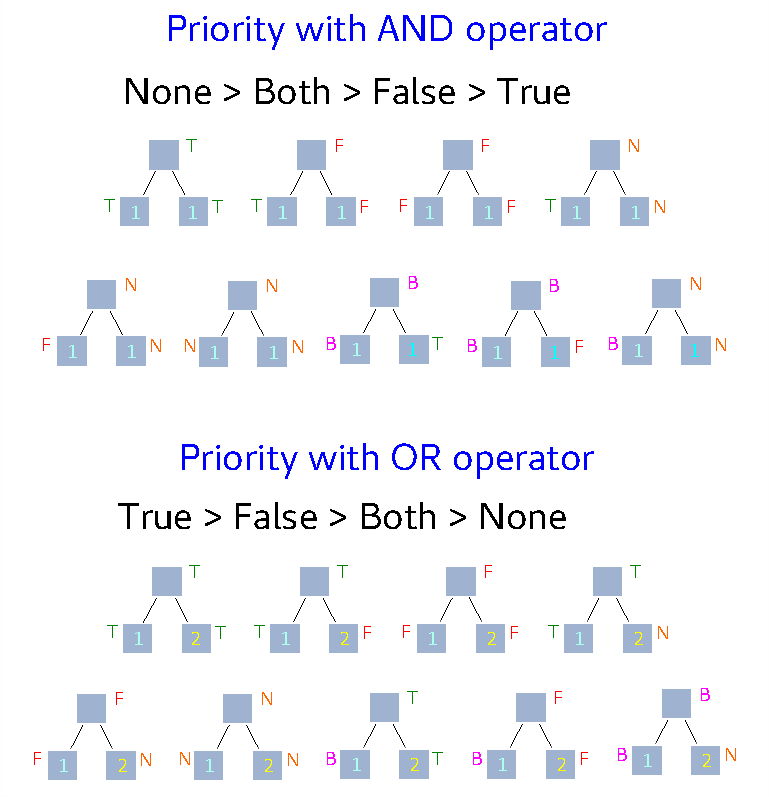
\includegraphics[width=\textwidth]{img/four_values_priorities_rules.pdf}
    \caption{ Règle de priorité pour l'inférence de multiple valeurs de vérité à travers un graphe "et/ou". }
    \label{fig:four_truth_values}
\end{shadedfigure}


\subsection{Application}
Ce travail a abouti sur une première implémentation qui a été présentée lors de la conférence \texttt{RULEML2015}. En plus de pouvoir raisonner avec une logique multi-valuée, le système est réactif à l'introduction de nouveaux faits de sorte que seules les nouvelles conséquences sont recalculées.

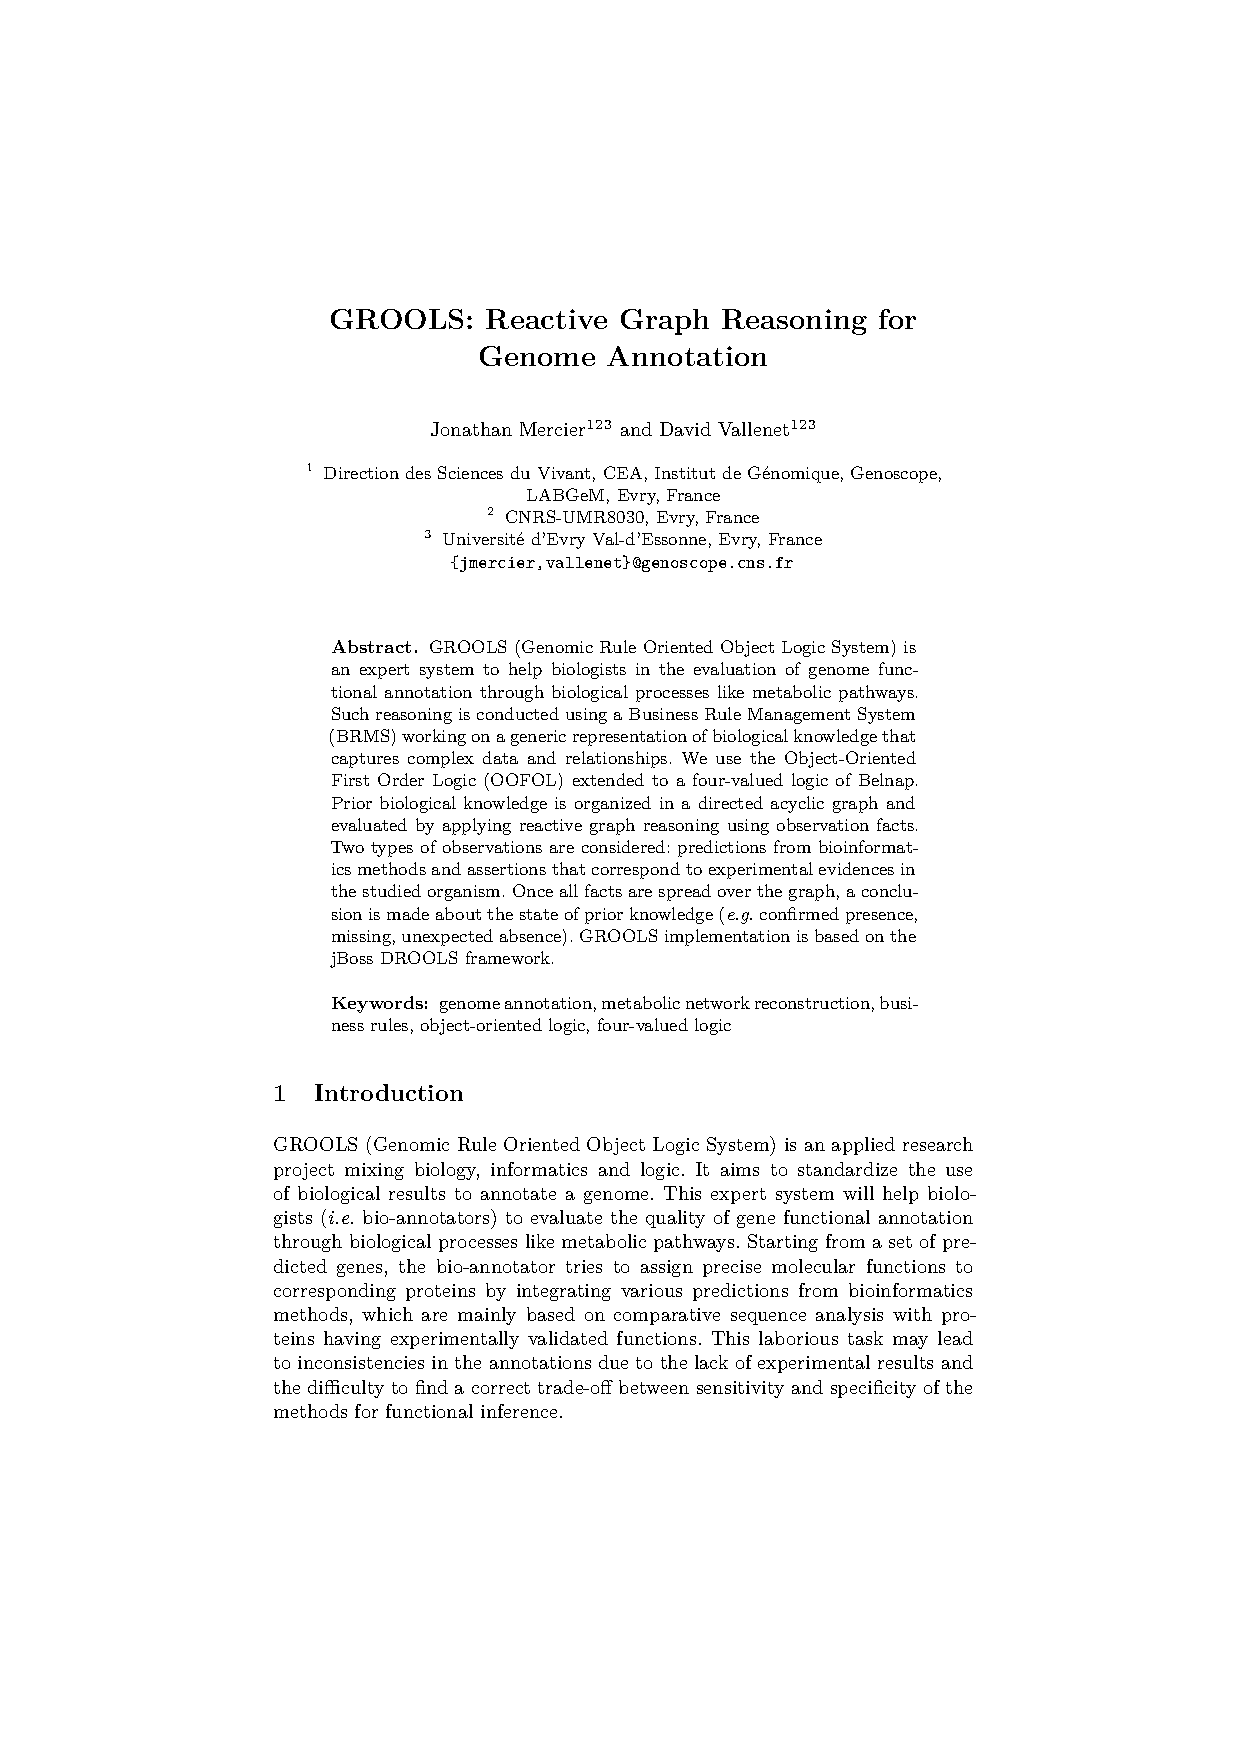
\includepdf[pages=-]{img/GROOLS__Reactive_Graph_Reasoning_for_Genome_Annotation.pdf}

\chapter{GROOLS: un système expert pour l'annotation fonctionnelle}

\section{Raisonnement sur des ensembles de valeurs de vérité}

La logique à quatre valeurs a ses limites lorsque l'on raisonne sur un graphe hiérarchique de connaissances. En effet, dans certains cas qui impliquent au moins deux concepts équivalents, il n'est pas possible de suggérer le chemin le plus plausible comme montré dans la \cref{fig:grools_belnap}. Bien que si on prête attention aux concepts feuilles du graphe (les unités fonctionnelles), intuitivement on choisirait le variant avec la plus grande proportion de fonctions prédites.

\begin{shadedfigure}[H]
	\begin{subfigure}[t]{.48\textwidth}
		\centering
		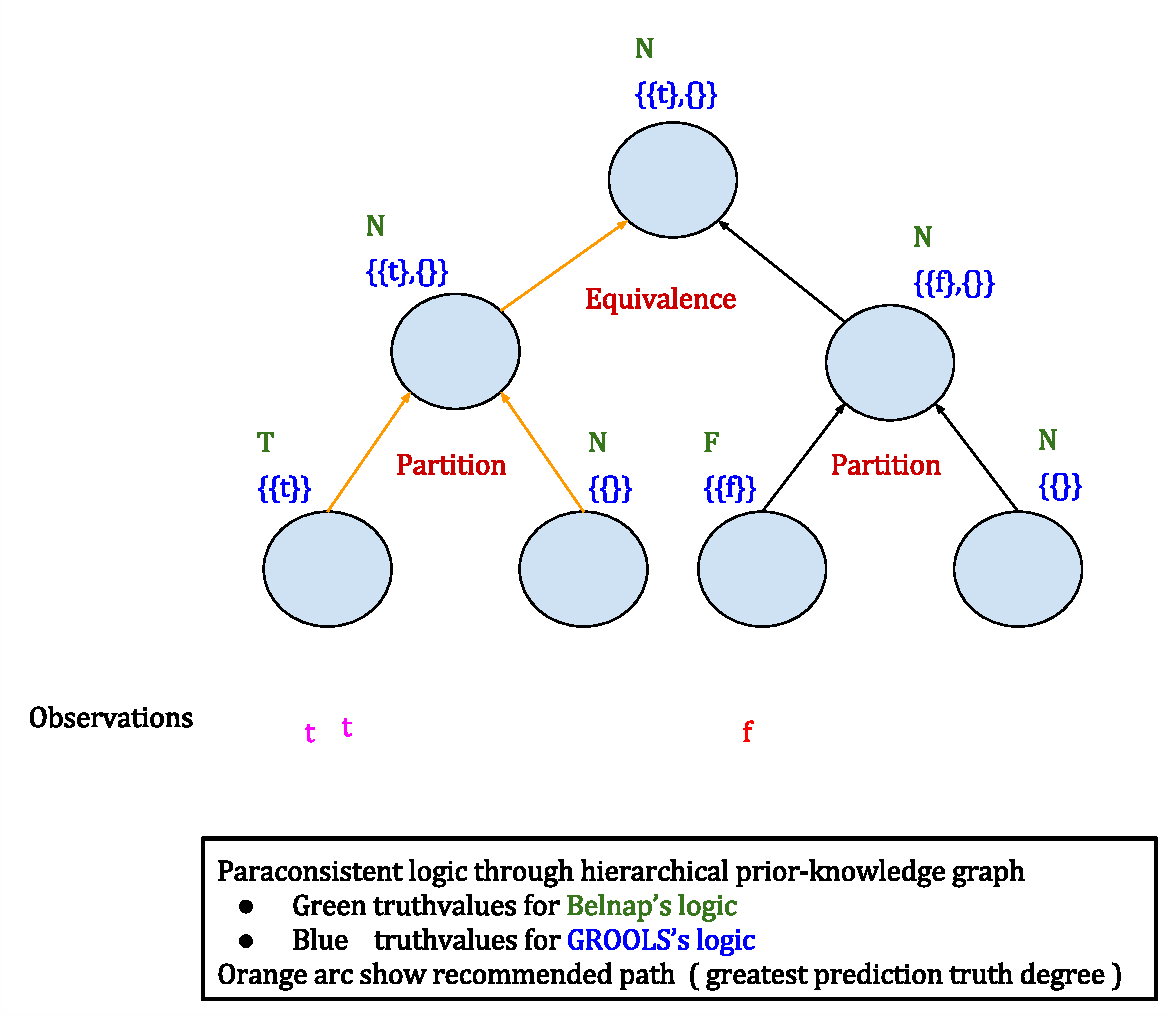
\includegraphics[width=\textwidth]{img/GROOLS_vs_belnap_1.pdf}
		\caption{Avec la logique de Belnap, il n'est pas possible de suggérer le chemin le plus vraisemblable lorsqu'il y a des valeurs incertaines.}
		\label{fig:grools_belnap_1}
	\end{subfigure}
	\hfill
	\begin{subfigure}[t]{.48\textwidth}
		\centering
		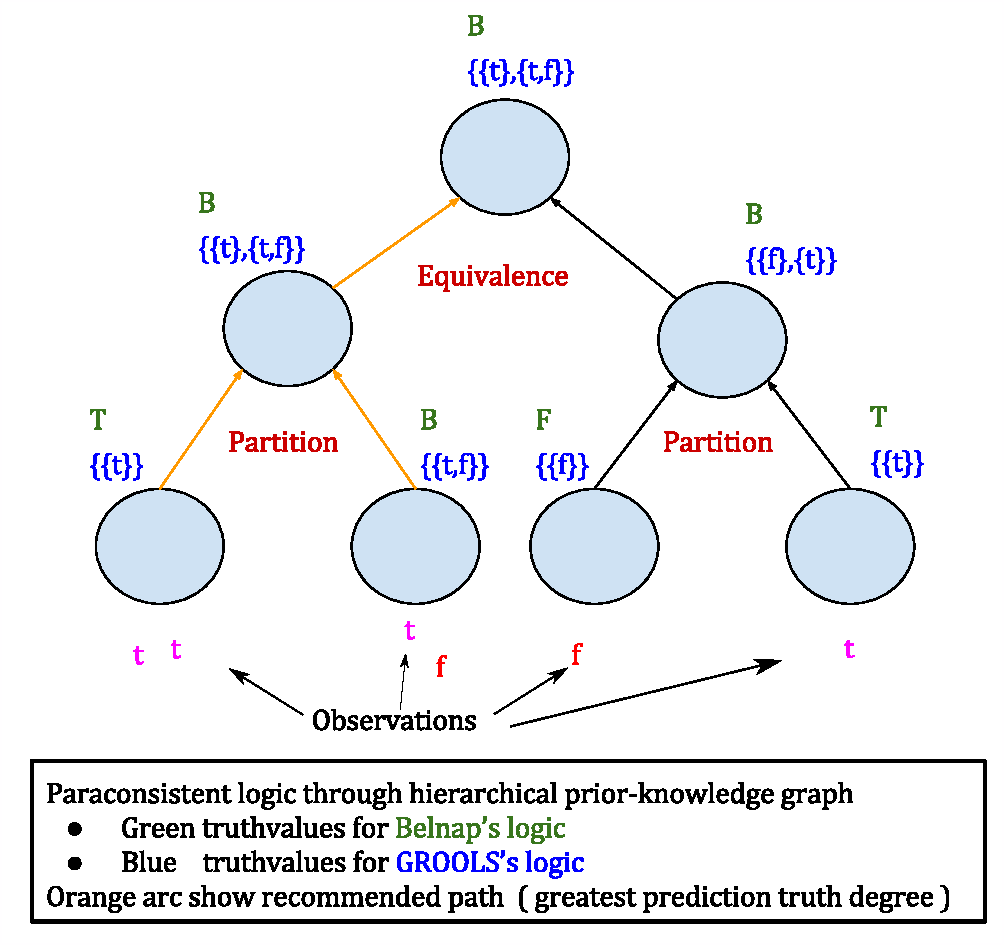
\includegraphics[width=\textwidth]{img/GROOLS_vs_belnap_2.pdf}
		\caption{Avec la logique de Belnap, il n'est pas possible de distinguer le chemin avec le plus grand degré de véracité. }
		\label{fig:grools_belnap_2}
	\end{subfigure}
	\label{fig:grools_belnap}
\end{shadedfigure}

J'ai réalisé que la notion de valeur contradictoire décrite par Belnap ("Both") était en fait un ensemble de valeurs de vérité vrai-et-faux. Par conséquent, essayer de représenter un ensemble de plusieurs valeurs dans une seule valeur de vérité "Both" est approximatif.

Sur la même idée, j'ai constaté que, dans mon cas d'application, j'avais des ensembles d'observations. En effet, des observations provenant de multiples sources peuvent désigner un même concept. D'autre part en laboratoire, on peut être amené à répéter une même expérience. Il y a également le cas de figure d'équipes différentes qui ont réalisé la même expérience. Dans ces deux cas, de multiples observations sont reliées a une même théorie. Elles peuvent avoir des résultats expérimentaux différents. Par conséquent, les ensembles de valeurs de vérité possibles en lien avec les ensembles d'observations sont : $\{t\} \{f\} \{t,f\} \{\emptyset\}$, respectivement ensemble : vrai, faux, vrai-et-faux, ni-vrai-ni-faux. 

Quant aux connaissances \textit{a priori}, elles sont observables par de multiples ensembles d'observations dus à la notion de composition de concepts. Pour illustrer, une connaissance \texttt{A} est composée d'une connaissance \texttt{B} et d'une autre \texttt{C}. Les observations relatives à la connaissance \texttt{A} sont l'union des ensembles d'observations de \texttt{B} et de \texttt{C}. C'est donc un ensemble d'ensembles\footnote{En anglais on utilise le terme de "powerset"} d'observations. La combinaison des quatre ensembles d'observations ($\mathbb{P}(2)$) donne seize ensembles ($\mathbb{P}(4)$). Ces seize combinaisons permettent de mieux représenter la population des observations liées à un concept. Ces ensembles permettent de faire des choix sans approximation lors du raisonnement. Peu de temps après avoir décrit cette combinatoire d'ensembles, j'ai remarqué l'existence d'un travail de recherche similaire réalisé par \citeauthor{shramko2005some}. Ils décrivent ces mêmes ensembles, nommés les valeurs de vérité généralisées. Ces valeurs ont été présentées dans la partie \nameref{par:logic_multivalued}  à travers la \cref{fig:sixteen_truth_values}.

\needspace{5\baselineskip}
\begin{tasks}[counter-format = {tsk[1].},label-offset = {0.8em},label-format = {\bfseries}](4)
	\task $\{\emptyset\}$
	\task $\{\{\emptyset\}\}$
	\task $\{\{t\}\}$
	\task $\{\{f\}\}$
	\task $\{\{t,f\}\}$
	\task $\{\{t\},\{t,f\}\}$
	\task $\{\{\emptyset\},\{t\}\}$
	\task $\{\{\emptyset\},\{f\}\}$
	\task $\{\{t\},\{f\}\}$
	\task $\{\{f\},\{t,f\}\}$
	\task $\{\{\emptyset\},\{t\},\{t,f\}\}$
	\task $\{\{t\},\{f\},\{t,f\}\}$
	\task $\{\{\emptyset\},\{t\},\{f\}\}$
	\task $\{\{\emptyset\},\{t,f\}\}$
	\task $\{\{\emptyset\},\{f\},\{t,f\}\}$
	\task $\{\{\emptyset\},\{t\},\{f\},\{t,f\}\}$
\end{tasks}

Les observations dans GROOLS sont dissociées en deux types : prédiction et expectation. Ainsi, chaque théorie possède deux espaces distincts (l'espace des prédictions et l'espace des expectations). Ces espaces sont représentés par des ensembles de valeurs de vérité $\mathbb{P}(4)$ . Les prédictions sont inférées vers les connaissances généralistes, c'est-a-dire des unités fonctionnelles vers les voies métaboliques et inversement pour les expectations. Lorsqu'au moins deux chemins équivalents se présentent, l'inférence des prédictions et des expectations peut être conditionnée selon le degré de véracité ou de fausseté. Par exemple, l'expectation d'une voie métabolique attendue sera propagée sur le ou les variants ayant des prédictions avec le plus grand degré de croyance : si un variant \texttt{A} est représenté par l'ensemble $\{\{t,f\}\}$ et un variant  \texttt{B} est représenté par l'ensemble $\{\{f\}\}$ alors le variant \texttt{A} est suggéré.

Un avantage de cette représentation en ensembles est la possibilité de calculer un degré de croyance, que l'on appelle également degré de véracité. Pour ce faire, le calcul est composé de quatre étapes et débute par les valeurs booléennes, c'est-à-dire les valeurs de vérités : vrai et faux. Le postulat de départ est le suivant : la valeur vrai "\texttt{t}"  vaut 1 sur l'échelle de la véracité et 0 pour la valeur faux "\texttt{f}".

\needspace{25\baselineskip}
\begin{enumerate}
    \item Constitution des ensembles $\mathbb{P}(2)$ (i.e $\{\emptyset\},\{t\},\{f\},\{t,f\}$)
    \item Calcul du degré de vérité pour les ensembles  $\mathbb{P}(2)$.
    \begin{equation*}
    \frac{1}{n} \sum_{i=1}x_{i}
    \begin{cases}
    \{\emptyset\} \to \frac{0}{1} = 0 \\
    \{t\} \to \frac{1}{1} = 1 \\
    \{f\} \to \frac{0}{1} = 0 \\
    \{t,f\} \to \frac{1+0}{2} = 0.5
    \end{cases}
    \end{equation*}
    \item Constitution des ensembles $\mathbb{P}(4)$ (i.e les 16 ensembles).
    \item Calcul du degré de vérité pour les ensembles  $\mathbb{P}(4)$ . Chaque sous-ensemble est représenté par son degré de vérité (ex: $\{\{t\}.verit\acute{e},\{f\}.verit\acute{e}\}$). Quelques exemples:
    \begin{equation*}
    \frac{1}{n} \sum_{i=1}x_{i}.verit\acute{e}
    \begin{cases}
    \{\{t\}\}                               &\to \frac{1}{1} = 1 \\
    \{\{t,f\}\}                             &\to \frac{1}{2} = 0.5 \\
    \{\{t\},\{t,f\}\}                       &\to \frac{1+0.5}{2} = 0.75 \\
    \{\{\emptyset\},\{t\}\}                 &\to \frac{0+1}{2} = 0.5 \\
    \{\{t\},\{f\}\}                         &\to \frac{1+0}{2} = 0.5 \\
    \{\{\emptyset\},\{t\},\{f\},\{t,f\}\}   &\to \frac{0+1+0+0.5}{4} = 0.125
    \end{cases}
    \end{equation*}
\end{enumerate}

Cette méthode permet de calculer également le degré de fausseté (i.e non-croyance). Pour des ensembles  $\mathbb{P}(2)$ et au delà, on peut calculer (i) le degré de contradiction (1 pour le sous-ensemble $\{t,f\}$ et 0 pour les autres), (ii) le degré d'incertitude (1 pour le sous-ensemble $\{\emptyset\}$ et 0 pour les autres).

\begin{shadedfigure}[H]
    \centering
    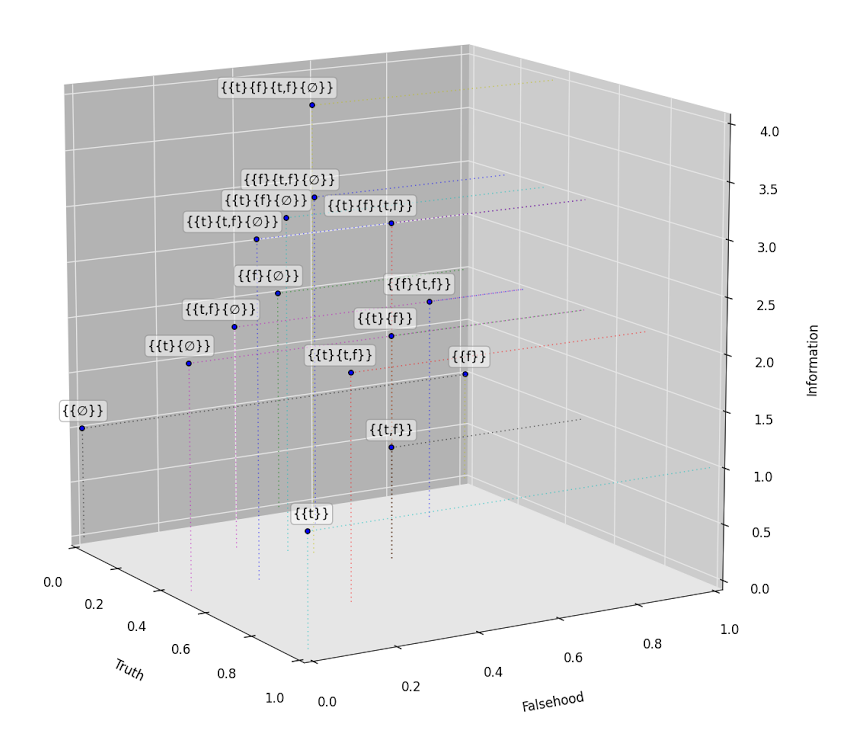
\includegraphics[width=\textwidth]{img/set_3d.png}
    \caption{Représentation des ensembles  $\mathbb{P}(4)$ selon 3 axes, (i) vérité, (ii) fausseté, (iii) information (i.e le nombre de sous-ensembles).}
    \label{fig:set3d}
\end{shadedfigure}

\section{La méthode GROOLS}\label{sec:methode}

Mes recherches m'ont conduit à développer une méthode pour représenter et raisonner sur des ensembles de valeurs de vérité. Ces ensembles sont utilisés pour décrire les prédictions et les expectations des différentes théories.

J'ai développé un système expert, nommé \texttt{\gls{GROOLS}}, utilisant une logique paracohérente pour assister le biocurateur dans le processus de l'annotation fonctionnelle des protéines. \texttt{\gls{GROOLS}} permet d'évaluer la complétion et la cohérence des fonctions prédites au travers des processus biologiques comme des voies métaboliques. A la fin du raisonnement, la méthode émet des conclusions sur les différents composants des processus. Par l'utilisation d'expectations envers l'organisme étudié, ces conclusions permettent d'informer le biologiste sur les composants confirmés, manquants, ambigus, etc. La méthode et les résultats sont décrits dans l'article suivant.

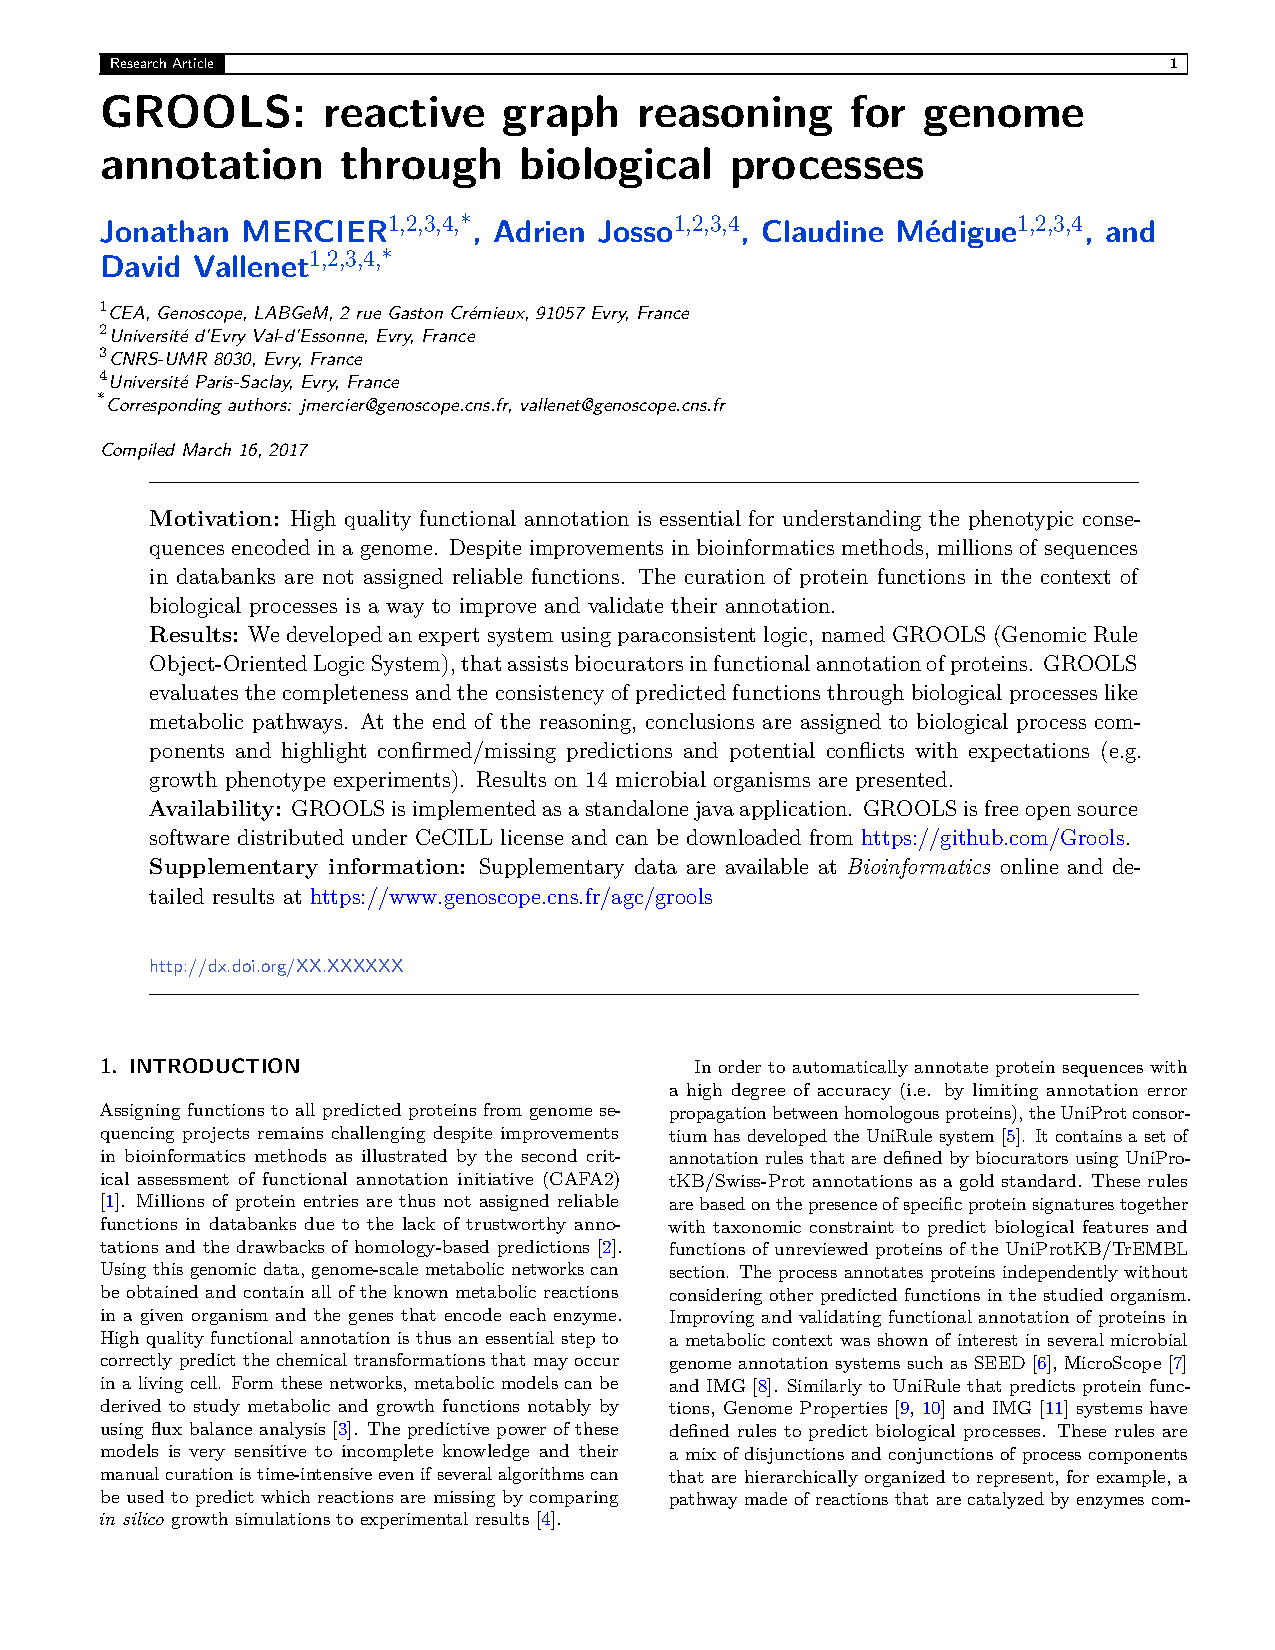
\includepdf[pages=-]{img/GROOLS_bioarchiv.pdf}

\section{Discussion}
\subsection{Difficultés rencontrées}
L'implémentation du raisonnement dans le moteur de règles \texttt{DROOLS} a engendré quelques difficultés. La première est la non maîtrise du moment de l'évaluation d'un groupe de faits par une règle. Il faut savoir que seul le moteur de règle décide quelle règle doit être activée à tel moment. Les conflits de priorités entre les règles sont gérés par \texttt{DROOLS} en interne par un système de résolution de conflits. Il arrive, par exemple, que deux règles peuvent s'activer à un même moment car elles évaluent les mêmes faits. Pour illustrer un tel cas, considérez les deux règles suivantes:

\needspace{25\baselineskip}
\begin{lstlisting}[style=drl-style,caption=conflit]
rule "Direct prediction"
when
	$k : PriorKnowledge(  )
	$p : Observation( type = Type.PREDICTION,  value != $k.prediction )
then
	modify($k){
		prediction = $p.value
	}
end

rule "Infer prediction from children PriorKnowledge"
when
	$k    : PriorKnowledge(  )
	$child: PriorKnowledge( $k memberOf parents, prediction not in $k.prediction )
then
	modify($k){
		prediction += $child.prediction
	}

end
\end{lstlisting}

Ces deux règles vont se déclencher dès qu'une connaissance \textit{a priori} est ajoutée ou mise à jour. Par contre, l'ordre de déclenchement n'est pas maitrisable ce qui peut changer complétement le résultat. Par exemple, en supposant que la connaissance \textit{a priori}  possède une prédiction $\{\{t,f\}\}$, le concept enfant  $\{\{f\}\}$ et l'observation $\{\{t\}\}$, si la règle 1 se déclenche avant la 2 alors la prédiction sera $\{\{t\},\{t,f\}\}$. En revanche, si la règle 2 est activée avant, on obtient la prédiction  $\{\{t\}\}$.

Il existe le système de "\texttt{salience}" qui attribue un poids à une règle et ainsi priorise les règles les unes par rapport aux autres.  Cependant, avoir recours à la "\texttt{salience}" est souvent le signe d'un raisonnement mal formulé.

De plus dans un système réactif, la modification de la connaissance \textit{a priori} induite par les deux règles précédentes provoque une boucle dans le raisonnement car elles vont perpétuellement s'activer réciproquement. Pour éviter de tels cas de figure, il est nécessaire de rendre les règles plus précises. Pour cela, de nouvelles règles doivent être ajoutées afin de couvrir la diversité des problèmes. En conséquence, il y a un risque plus important de collision de règles. À chaque nouvel ajout de règles, il faut s'assurer de l'absence de conflit vis-à-vis de toutes les autres règles et de la diversité des faits possibles. Tout ceci rend la construction d'un raisonnement réactif très compliqué. Dans le cas précédemment décrit, la règle  pour l'inférence de la  prédiction "directe"  peut être divisée en deux règles : la première pour inférer l'ensemble des observations lorsque la connaissance \textit{a priori} ne possède aucune prédiction ($\{\{\emptyset\}\}$) et une seconde lorsque la connaissance \textit{a priori} possède au moins une prédiction, les observations directes viennent s'ajouter à l'ensemble des prédictions.

Une des grandes difficultés lorsque l'on travaille avec ce type d'outil, c'est que nous obtenons un résultat final sans être en mesure d'identifier quelles règles ont été activées et pourquoi elles l'ont été. Le système \texttt{DROOLS} fournit un système de trace des évènements mais il est compliqué à analyser. Il n'indique pas pourquoi la règle est activée et encore moins pourquoi elle n'a pas été activée. En effet, même pour un petit jeu de données, les traces produisent un volume important d'évènements, ce qui demande du temps pour les analyser et comprendre les choix du raisonneur. Il est donc extrêmement laborieux d'analyser les traces, par exemple, certains cas non souhaités sont dus à l'activation d'une succession de règles.

En plus des difficultés pour coordonner les différentes règles, j'ai rencontré des erreurs critiques dans le système \texttt{DROOLS}. Ces problèmes ont été rapportés aux développeurs quand j'étais en mesure de fournir un exemple minimal reproduisant le bug. Ci-dessous, je présente deux bugs que j'ai découvert avec la description d'un cas minimal, rapportés à l'équipe de développement de \texttt{DROOLS}:
\begin{itemize}
	\item \url{https://issues.jboss.org/browse/DROOLS-809}
	\item \url{https://issues.jboss.org/browse/DROOLS-809}
\end{itemize}
 
En plus de devoir exprimer des règles sans conflit les unes par rapport aux autres, le système me contraignait sur la façon dont je pouvais les exprimer à cause de ces "bugs" rencontrés.

Malgré toutes ces difficultés, ce travail a abouti à une version fonctionnelle, accessible à l'adresse : \url{https://github.com/Grools/grools-drools-checker} . Cependant, le raisonneur \texttt{DROOLS} a montré ses limites pour raisonner sur des données hiérarchiques. Les règles et les faits ne sont pas utilisés dans un ordre optimum vis-à-vis du graphe de connaissances. De nombreuses ré-activations de règles sont observées, induisant un temps de calcul accru. De plus, l'évaluation de collections de faits (essentielle pour le raisonnement) est très couteuse pour le raisonneur \texttt{DROOLS}. Ces opérations empêchent le raisonneur d'activer les règles de façon efficace. Elles peuvent s'écrire avec les expressions suivantes : \lstinline[style=drl-style]$Set() from collect(...)$, \lstinline[style=drl-style]$forall(...)$, \lstinline[style=drl-style]$Number() from accumulate(...)$\footnote{Des exemples sur ces expressions sont accessibles à l'adresse suivante: \url{http://blog.athico.com/2007/06/chained-from-accumulate-collect.html}.}. Ces instructions recréent des collections d'objets à chaque réactivation d'une règle, ce qui est inefficace. Ainsi, le raisonnement prend entre deux et neuf heures de calcul selon la quantité de faits et la représentation des connaissances utilisées (\texttt{Genome Properties} ou UniPathway). Il était donc nécessaire d'ajouter des règles permettant d'ordonner l'activation des règles dédiées au raisonnement et, ainsi, minimiser le nombre de réactivations vis-à-vis du graphe de connaissances. J'avais commencé ce travail, mais là encore, j'ai été confronté à des comportements indésirables de la part du raisonneur. J'ai établi au cours de ces trois années de bonnes relations avec l'équipe de développement de \texttt{DROOLS} . À la suite de la présentation  des nouveaux problèmes rencontrés, ils m'ont proposé de travailler conjointement pour apporter des corrections dans la version suivante. Malheureusement, le temps qui m'était imparti ne me permettait pas d'investiguer dans le moteur d'inférence de DROOLS, de trouver une solution, de la faire valider et d'attendre la nouvelle version.

C'est la raison pour laquelle, j'ai ré-écrit un moteur de raisonnement réactif dans le langage Java. Afin de rester dans le contexte d'une programmation déclarative, les règles ont été écrites en utilisant le paradigme de la programmation fonctionnelle\footnote{\url{https://fr.wikipedia.org/wiki/Programmation_déclarative}}. Ce projet open source est appelé \texttt{grools-reasoner} (\url{https://github.com/Grools/grools-reasoner}). Cette bibliothèque a été utilisée pour l'exploration des voies métaboliques de 14 génomes bactériens dans l'article présenté dans la \namecref{sec:methode} \cref{sec:methode}. L'outil s'est montré capable de raisonner sur tout un génome en moins d'une minute.

La bibliothèque est modulaire, elle peut être utilisée pour différents besoins :\nolisttopbreak
\begin{itemize}
	\item \texttt{grools-application}l'exploration du métabolisme à travers les modèles \texttt{Genome Properties} et \texttt{UniPathway}  (\url{https://github.com/Grools/grools-application}).
	\item \texttt{grools-interpreter}charger un ancien raisonnement et effectuer des requêtes pour l'analyse des faits (\url{https://github.com/Grools/grools-interpreter}).
	\item et d'autres à venir\ldots
\end{itemize}

\subsection{Logique paracohérente}
Lorsqu'il est nécessaire de raisonner dans un monde avec des incertitudes et des incohérences, la logique à quatre valeurs de \textit{Belnap} semble suffisante. En effet, les valeurs de vérités TRUE, FALSE, BOTH et NONE couvrent la notion de vrai, faux, contradictoire et incertain. Cependant, lorsque l'on regarde de plus près la table de vérité  (voir la section \nameref{par:logic_multivalued}  \cref{tab:belnap_truth_table}), certaines combinaisons peuvent se montrer contre-intuitives, par exemple: $ BOTH \lor  NONE = TRUE$ et $ BOTH \land NONE = FALSE$. Le premier cas  peut se représenter de la sorte: 
\begin{enumerate}
    \item Un variant \texttt{A} d'une voie métabolique possède des prédictions contradictoires (BOTH)
    \item Un autre variant \texttt{B} a une absence de prédiction (NONE)
    \item La voie métabolique va être prédite (TRUE), d'après la table de vérité de \textit{Belnap}, par le calcul de la proposition \texttt{A} OU \texttt{B}.
\end{enumerate}
Ce résultat non-intuitif est dû à une impossibilité d'exprimer plus de quatre états et ne peut pas, ainsi, faire la distinction entre des valeurs de vérité à part entière et des ensembles de valeurs de vérité. Cette logique essaye de représenter l'ensemble $\{t,f\}$ qui comporte deux valeurs en une seule, ce qui inexorablement amène à des approximations. Cette logique ne peut donc pas être utilisée avec un graphe de connaissances sans amener des  imprécisions comme montré avec la \cref{fig:grools_belnap_1} et la  \cref{fig:grools_belnap_2}. 

Mon interprétation est que ces ensembles de valeurs de vérité ne sont pas des valeurs de vérité. Par conséquent, il ne faut pas essayer d'étendre la logique classique à d'autres valeurs de vérités. Ce point de vue rejoint celui émis par \citeauthor{dubois2008ignorance} dans \citetitle{dubois2008ignorance}\cite{dubois2008ignorance}. La logique multi-valuée de Belnap a introduit une confusion entre valeur de vérité et l'état d'information.


\end{refsegment}
